\documentclass[xetex,mathserif,serif]{beamer}
\usepackage{fontspec}
\usepackage{xunicode} %Unicode extras!
\usepackage{xltxtra}  %Fixes
\setmainfont{Source Sans Pro}
\usepackage{blindtext}
\usetheme{polymtl}
\defaultfontfeatures{Scale=MatchLowercase,Mapping=tex-text}
\setbeamertemplate{itemize items}[default]
\setbeamertemplate{enumerate items}[default]
\title{\textbf{nrw.uniTS}\\ Private Daten schützen}
\author{Philipp Deppenwiese}

\begin{document}

	\frame{\titlepage}
	\begin{frame}
		\begin{block}{Chaos Computer Club}
			\texttt{Öffentliche Daten nützen, private Daten schützen.}
		\end{block}
	\end{frame}	
	
	\begin{frame}
	
\includegraphics[scale=0.1]{./nsa.png}
	\end{frame}
	
	\begin{frame}
	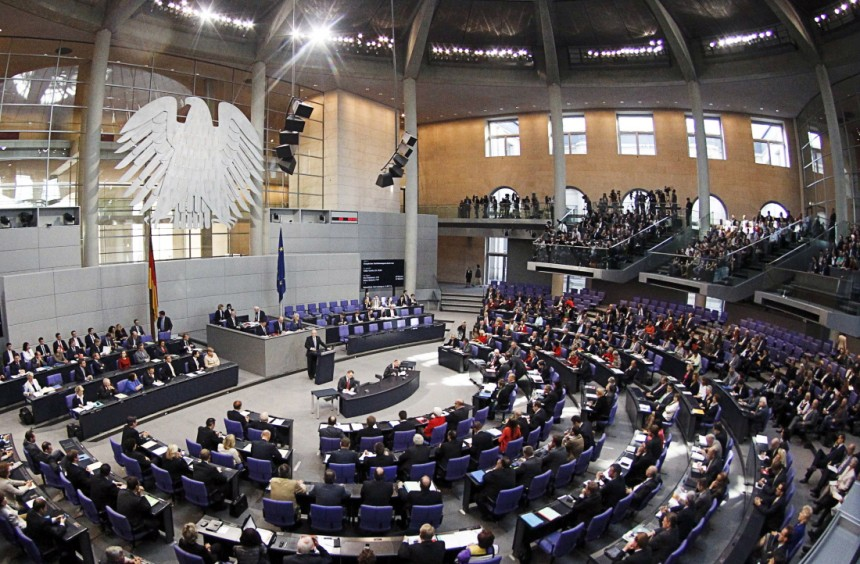
\includegraphics[scale=0.3]{./bundestag.jpg}
	\end{frame}
	
	\begin{frame}
	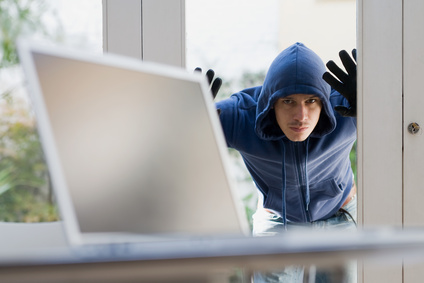
\includegraphics[scale=0.6]{./laptop_klau.jpg}
	\end{frame}
	
	\begin{frame}
	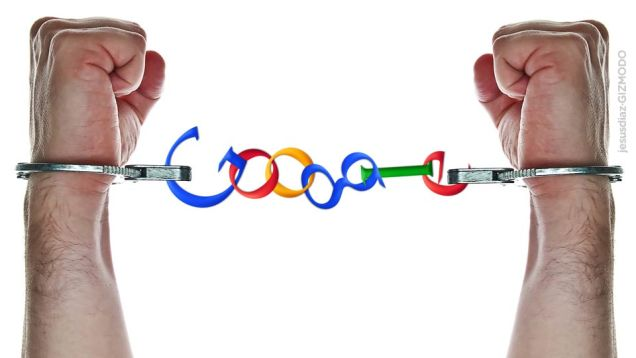
\includegraphics[scale=0.9]{./google.jpg}
	\end{frame}
	
	\begin{frame}
		\tableofcontents
	\end{frame}
	\section{EMail-Verschlüsselung}
	\subsection{Anwendungfälle}
		\begin{frame}
		
		\end{frame}
	\subsection{Beispiele}
		\begin{frame}
		\blindtext
		\end{frame}
	\subsection{Zusammenfassung}
		\begin{frame}
		\blindtext
		\end{frame}
	\section{Festplattenverschlüsselung}



	\begin{frame}
		\begin{itemize}
			\item 2 Pac
			\item ODB
			\item Snoop Dog
		\end{itemize}
	\end{frame}

	\begin{frame}
		\begin{description}
			\item[ODB] Ol' Dirty Bastard.
			\item[NWA] Niggaz Wit Attitudes.
%			\item[
		\end{description}
		\end{frame}

	\begin{frame}
		\begin{block}{Definition}
			This is a defintion of some sort.
		\end{block}
	\end{frame}

	\begin{frame}
		\begin{theorem}[RZA, 1993]
			Wu-tang clan ain't nothin' to fuck wit.
		\end{theorem}
	\end{frame}
\end{document}
